\documentclass[a4paper,11pt,twoside,ngerman,color]{book}
\usepackage[a4paper,left=3.5cm,right=2.5cm,bottom=3.5cm,top=3cm]{geometry}

\usepackage[german,english]{babel}

\usepackage[pdftex]{graphicx,color}
\usepackage{amsmath,amssymb,subfigure}

% Theorem-Umgebungen
\usepackage[amsmath,thmmarks]{ntheorem}

% Korrekte Darstellung der Umlaute
\usepackage[utf8]{inputenc}
\usepackage[T1]{fontenc}

% Codeabschnitte
\usepackage{listings}
\usepackage{lstlinebgrd}

\definecolor{mygreen}{rgb}{0,0.6,0}
\definecolor{mygray}{rgb}{0.5,0.5,0.5}
\definecolor{mymauve}{rgb}{0.78,0,0.72}

\definecolor{design1}{HTML}{639ACE}
\definecolor{design2}{HTML}{53972F}
\definecolor{design3}{HTML}{C33F4F}
\definecolor{design4}{HTML}{DC8C46}
\definecolor{design5}{HTML}{4A34A8}

\lstset{ %
	backgroundcolor=\color{white},   % choose the background color
	basicstyle=\ttfamily\footnotesize,        	 % size of fonts used for the code
	breaklines=true,                 % automatic line breaking only at whitespace
	captionpos=b,                    % sets the caption-position to bottom
	commentstyle=\color{mygreen},    % comment style
	escapeinside={\%*}{*)},          % if you want to add LaTeX within your code
	keywordstyle=\color{blue},       % keyword style
	stringstyle=\color{mymauve},     % string literal style
	frame=single,
	showstringspaces=false,
	tabsize=2,
	numbers=left
}

\lstdefinelanguage{MyC++} {
	language=C++,
	morestring=[s]{/*}{*/},
}

% Bibtex deutsch
\usepackage[backend=biber]{biblatex}
\addbibresource{bibliography.bib}
\renewbibmacro{in:}{%
  \ifentrytype{inbook}{}{\printtext{\bibstring{in}\intitlepunct}}}

% URLs
\usepackage{url}

% Caption Packet
\usepackage[margin=0pt,font=small,labelfont=bf]{caption}

% Zeichnen von Darstellungen
\usepackage{tikz}
\usepackage{pgfplots}
\usepackage{pgfplotstable}

\usetikzlibrary{positioning,calc}

% Hinzufügen weiterer Symbole
\usepackage{bbding}

% Zeilenabstand einstellen %
\renewcommand{\baselinestretch}{1.25}

% Floating-Umgebungen anpassen %
\renewcommand{\topfraction}{0.9}
\renewcommand{\bottomfraction}{0.8}

% Abkürzungen richtig formatieren %
\usepackage{xspace}
\newcommand{\vgl}{vgl.\@\xspace} 
\newcommand{\zB}{z.\nolinebreak[4]\hspace{0.125em}\nolinebreak[4]B.\@\xspace}
\newcommand{\bzw}{bzw.\@\xspace}
\newcommand{\dahe}{d.\nolinebreak[4]\hspace{0.125em}h.\nolinebreak[4]\@\xspace}
\newcommand{\etc}{etc.\@\xspace}
\newcommand{\evtl}{evtl.\@\xspace}
\newcommand{\ggf}{ggf.\@\xspace}
\newcommand{\bzgl}{bzgl.\@\xspace}
\newcommand{\so}{s.\nolinebreak[4]\hspace{0.125em}\nolinebreak[4]o.\@\xspace}
\newcommand{\iA}{i.\nolinebreak[4]\hspace{0.125em}\nolinebreak[4]A.\@\xspace}
\newcommand{\sa}{s.\nolinebreak[4]\hspace{0.125em}\nolinebreak[4]a.\@\xspace}
\newcommand{\su}{s.\nolinebreak[4]\hspace{0.125em}\nolinebreak[4]u.\@\xspace}
\newcommand{\ua}{u.\nolinebreak[4]\hspace{0.125em}\nolinebreak[4]a.\@\xspace}
\newcommand{\og}{o.\nolinebreak[4]\hspace{0.125em}\nolinebreak[4]g.\@\xspace}
\newcommand{\oBdA}{o.\nolinebreak[4]\hspace{0.125em}\nolinebreak[4]B.\nolinebreak[4]\hspace{0.125em}d.\nolinebreak[4]\hspace{0.125em}A.\@\xspace}
\newcommand{\OBdA}{O.\nolinebreak[4]\hspace{0.125em}\nolinebreak[4]B.\nolinebreak[4]\hspace{0.125em}d.\nolinebreak[4]\hspace{0.125em}A.\@\xspace}

% Leere Seite ohne Seitennummer, naechste Seite rechts
\newcommand{\blankpage}{
 \clearpage{\pagestyle{empty}\cleardoublepage}
}

% Keine einzelnen Zeilen beim Anfang eines Abschnitts (Schusterjungen)
\clubpenalty = 10000
% Keine einzelnen Zeilen am Ende eines Abschnitts (Hurenkinder)
\widowpenalty = 10000 \displaywidowpenalty = 10000

% Formatierung von Paragraphen
\setlength{\parskip}{1pt}

% Hyperref-Paket zur Optimierung der PDF
\usepackage{hyperref}

\usepackage[markcase=noupper,headsepline]{scrlayer-scrpage}
\pagestyle{scrheadings}
\clearpairofpagestyles

\setkomafont{pagehead}{\normalfont}

\ohead{\pagemark}
\ihead{\headmark}
\automark[chapter]{chapter}

\hypersetup{
	pdftitle = {Effiziente String-Verarbeitung in Datenbankanfragen auf hochgradig paralleler Hardware},
	pdfauthor = {Florian Lüdiger},
	colorlinks=true,
	allcolors = black
}



\begin{document}
	\selectlanguage{german}
	
	\begin{titlepage}
\definecolor{TUGreen}{rgb}{0.517,0.721,0.094}
\vspace*{-2cm}
\newlength{\links}
\setlength{\links}{-1.5cm}
\sffamily
\hspace*{\links}
\begin{minipage}{12.5cm}

\includegraphics[width=8cm]{bilder/tud_logo_rgb}
%\hspace*{-0.25cm} \textbf{TECHNISCHE UNIVERSIT"AT DORTMUND}\\
%\hspace*{-1.2cm} \rule{5mm}{5mm} \hspace*{0.1cm} FACHBEREICH INFORMATIK\\
\end{minipage}

\vspace*{4cm}

\hspace*{\links}
\hspace*{-0.2cm}
\begin{minipage}{9cm}
\large
\begin{center}
{\Large Diplomarbeit} \\
\vspace*{1cm}
\textbf{Titel der Diplomarbeit} \\
\vspace*{1cm}
Name des Diplomanden\\
% \vspace*{1cm}
Monat der Abgabe
\end{center}
\end{minipage}
\normalsize
\vspace*{5.5cm}

% \hspace*{\links}

\vspace*{2.1cm}

\hspace*{\links}
\begin{minipage}[b]{5cm}
% \normalsize
\raggedright
Gutachter: \\
Name des Erstgutachters \\
Name des Zweitgutachters \\
\end{minipage}

\vspace*{2.5cm}
\hspace*{\links}
\begin{minipage}[b]{8cm}
% \normalsize
\raggedright
Technische Universit"at Dortmund \\
Fakult"at f"ur Informatik\\
Lehrstuhlbezeichnung (LS-Nummer)\\
http://lsXXX-www.cs.tu-dortmund.de
\end{minipage}
%%%%%%%%%%%%%%%%%%%%%%%%%%%%%%%%%%%%%%%%%%%%%%%%%%
% bei Kooperation mit anderen Lehrstuehlen,
% sonst weglassen
\begin{minipage}[b]{8cm}
% \normalsize
\raggedleft
In Kooperation mit:\\
Fakult"atsname\\
Lehrstuhl-/Institutsbezeichnung
\end{minipage}
%%%%%%%%%%%%%%%%%%%%%%%%%%%%%%%%%%%%%%%%%%%%%%%%%%

\end{titlepage}

	\blankpage
	
	\pagenumbering{roman}
	\tableofcontents
	\cleardoublepage
	
	\pagenumbering{arabic}
	
	% Kapitel
	\chapter{Einleitung}

Ein Großteil der Datensätze, die in realen Systemen zum Einsatz kommen enthalten eine große Vielfalt an String-Datensätzen mit verschiedensten Eigenschaften.
Die Operationen, die auf diesen Datensätzen ausgeführt werden reichen von Gleichheitsüberprüfungen über das Enthaltensein eines Teilstrings bis zum Erfüllen eines komplexen, regulären Ausdrucks.
In dieser Arbeit wird untersucht werden, wie sich die unterschiedlichen Operationen zur String-Verarbeitung verhalten, wenn diese auf einer hochgradig parallel arbeitenden Grafikkarte ausgeführt werden.
Außerdem wird analysiert, ob ein Verfahren zur Steigerung der Auslastung der Grafikkarte eine signifikante Leistungssteigerung erzielen kann.

\section{Motivation und Hintergrund}

Die effiziente Berechnung unterschiedlicher Operatoren auf Zeichenketten ist essenziell für das Erreichen eines hohen Durchsatzes und für das Gewährleisten von maximaler Performanz.
In diesem Kontext versprechen Grafikkarten durch ihre hochgradig parallele Architektur in der Theorie eine bestmögliche Leistung.

Der Aufbau von moderner, hoch paralleler Hardware wie einer Grafikkarte führt dazu, dass diese besonders effizient mit gleichmäßigen Daten arbeiten kann.
Ein String-Datensatz ist dagegen typischerweise sehr heterogen durch die unterschiedlichen Längen der einzelnen Zeichenketten, wodurch das Verarbeiten auf einer Grafikkarte zunächst einige Schwierigkeiten birgt.
Aus diesem Grund verwenden bisherige Ansätze zur Verarbeitung von Zeichenketten das Konzept der Dictionaries \cite{Mueller2014}.
Dabei wird eine Tabelle mit allen Strings aufgebaut und zu diesen ein Schlüssel abgespeichert, welcher zusammen mit jedem String in den anderen Tabellen der Datenbank gespeichert wird.
Somit können String-Operationen durch andere Operationen auf den Schlüsseln abgebildet werden, wodurch diese eine einheitliche Struktur und damit ein effizientes Ausführungsmuster auf Grafikkarten erhalten.
Das Aufbauen und Verwalten des für diese Technik verwendeten Dictionaries erzeugt vor allem bei Daten, die sich häufig ändern, einen hohen Aufwand, wodurch die Leistungsfähigkeit des Gesamtsystems sinkt.
Um diesen Verwaltungsaufwand für eine zusätzliche Datenstruktur zu eliminieren, wäre es wünschenswert eine Lösung zu finden, die den Verwaltungsaufwand eliminiert und direkt auf den ursprünglichen String-Daten arbeitet.

Soll eine komplexere Operation auf den Daten ausgeführt werden, die mit regulären Ausdrücken arbeitet, ist die Verwendung eines Dictionaries nicht mehr möglich und spätestens an dieser Stelle muss auf eine andere Methode zurückgegriffen werden.
Die Verwendung von regulären Ausdrücken eröffnet in vielen Anwendungsfällen verschiedenste Möglichkeiten, String-Daten effizient zu verarbeiten und die Leistungsfähigkeiten des Datenbanksystems voll auszunutzen.
Reguläre Ausdrücke stellen ein mächtiges Werkzeug dar, welches den meisten Anwendern von Datenbankmanagementsystemen bekannt ist und vor allem relevant ist, da es das hoch effiziente Auswerten komplexer Muster erlaubt.

Die meisten aktuellen Datenbankmanagementsysteme bieten eine Unterstützung für reguläre Ausdrücke, da sie das effiziente Abgleichen komplexer Muster ermöglichen und dabei eine hohe Leistung garantieren.
Gäbe es eine solche Funktion nicht, müsste eine entsprechende Selektion nach dem Ausführen des Anfrageplans durch das DBMS manuell im Anwendungsprogramm durchgeführt werden.
An dieser Stelle entstehen zahlreiche Probleme, da der Optimierer die Selektion nicht an der optimalen Stelle im Anfrageplan platzieren kann, damit frühzeitig Tupel weg fallen, die nicht in das Ergebnis aufgenommen werden.
Es entsteht also schon beim Datenbankserver eine erhöhte Last durch das unnötige Verarbeiten von Tupeln.
Diese werden zusätzlich noch über das Netzwerk zur Anwendung übertragen, wodurch erneut eine erhöhte Netzlast entsteht.
Die Anwendung wiederum muss anschließend mit einer potenziell geringeren Leistungsfähigkeit als der Datenbankserver die Selektion durchführen, wodurch an dieser Stelle wieder eine unnötig hohe Last entsteht.
Sollten also Anwendungsfälle auftreten, bei denen eine Selektion durch reguläre Ausdrücke gewünscht ist, stellt die Unterstützung dieser Operation durch das Datenbankmanagementsystem einen massiven Vorteil dar.
Auch für Datenbanksysteme, die auf Grafikkarten arbeiten sollte also sichergestellt sein, dass diese die maximal mögliche Performanz bei der Verarbeitung von regulären Ausdrücken erreichen.

\section{Zielsetzung}

In dieser Arbeit sollen verschiedene Operationen, die auf String-Daten arbeiten im Kontext von kompilierten Anfrageplänen mithilfe des Query Compilers DogQC untersucht werden.
Ziel ist es dabei die Performanz der umgesetzten Operatoren zu analysieren und Flaschenhälse, die durch eine schlechte Auslastung der Grafikkarte entstehen, zu identifizieren.
Diese Flaschenhälse sollen mithilfe des Lane Refill-Verfahrens eliminiert werden, wodurch eine Steigerung der Leistungsfähigkeit erreicht werden soll.
Neben einfachen String-Operatoren sollen auch komplexere Techniken, welche reguläre Ausdrücke zur String-Verarbeitung verwenden, analysiert werden und untersucht werden, ob diese einen Laufzeitgewinn durch das Lane Refill erreichen.
Mithilfe dieser Betrachtungen sollen Rückschlüsse darüber gezogen werden, ob das Lane Refill, welches bereits bei der Durchführung von Join-Operationen erfolgreich eingesetzt wird, auch für die Verarbeitung von Zeichenketten einen Nutzen bringt.

\section{Aufbau der Arbeit}

Um verstehen zu können, warum bei der Verarbeitung von String-Daten auf Grafikkarten verschiedene Probleme auftreten können, werden zunächst der Grundaufbau und die wichtigsten Eigenschaften von Grafikprozessoren erklärt.
Anschließend werden die bei DogQC zum Einsatz kommenden Verfahren zur Kompilierung von Anfrageplänen erläutert und die Rahmenbedingungen für die nachfolgenden Untersuchungen festgelegt.
In Kapitel \ref{sec:equals_naiv} wird der einfache String-Vergleich erarbeitet und auf verschiedene Probleme hingewiesen, die im nachfolgenden Kapitel durch den Einsatz des Lane Refill beseitigt werden.
An dieser Stelle wird außerdem erklärt, wie das Lane Refill-Verfahren funktioniert und warum es durch eine höhere Auslastung der Grafikkarte eine bessere Performanz erreichen kann.
Anschließend wird in Kapitel \ref{sec:regex} vorgestellt, wie reguläre Ausdrücke mithilfe von endlichen Automaten ausgewertet werden können und ein geeigneter Ansatz für die Umsetzung im Query Compiler ausgewählt.
Im folgenden Teil wird der parallele Musterabgleich mit regulären Ausdrücken umgesetzt und ähnlich wie beim einfachen String-Vergleich durch das Lane Refill erweitert.
Vorbereitend auf die im letzten Teil der Arbeit durchgeführten Leistungstests der verschiedenen Algorithmen wird aufgezeigt, wie das Optimieren verschiedener Parameter bei der Ausführung von Algorithmen auf einer Grafikkarte einen Einfluss auf die Performanz des Systems nimmt und wie diese Optimierung durchgeführt werden kann.
Schließlich folgen zwei Kapitel zur Evaluation des einfachen String-Vergleichs und des Musterabgleichs mit regulären Ausdrücken, in denen untersucht wird, wie sich die unterschiedlichen Algorithmen verhalten und ob durch die Verwendung des Lane Refill-Verfahrens ein Laufzeitgewinn erreicht werden kann.
Abschließend wird in einem Fazit Stellung dazu genommen, ob die hier beschriebene Zielsetzung erreicht werden konnte und ob das Lane Refill bei der Verarbeitung von Zeichenketten eine sinnvolle Anwendung findet.
	\chapter{Grundlagen des verwendeten Verfahrens}

\section{Grundlagen zu Grafikkarten und deren Programmierung}

\section{Das Lane-Refill-Verfahren}

	\chapter{Einfacher, paralleler String-Vergleich}

\section{Naive Umsetzung}

\section{Umsetzung mit Lane Refill}

\section{Verwendete Workloads und deren Merkmale}

\section{Vorstellung der Messergebnisse}

\section{Diskussion der Ergebnisse}

	\chapter{Grundlagen von regulären Ausdrücken}

Reguläre Ausdrücke sind ein Mittel, um ein Muster von Zeichenketten zu beschreiben.
Alle Wörter, die dem so beschriebenen Muster entsprechen, werden in einer sogenannten \emph{Sprache} zusammengefasst.
Erlaubte Operatoren innerhalb von regulären Ausdrücken sind beispielsweise die Konkatenation durch Aneinanderreihen von Elementen, Wiederholung durch den \texttt{*}-Operator, Auswahl durch den \texttt{|}-Operator oder das Verwenden einer Wildcard.

Das Überprüfen, ob ein Wort Teil der Sprache ist, die durch einen regulären Ausdruck beschrieben wird, wird \emph{Wortproblem} genannt.
Um dieses zu lösen wird ein endlicher Automat verwendet, welcher aus dem regulären Ausdruck generiert wird und durch einen gerichteten Graphen repräsentiert wird.
Die Knoten des Graphen werden auch Zustände genannt, wobei genau ein Zustand als Startzustand definiert wird und mindestens ein Zustand als akzeptierender Zustand ausgewählt wird.
Jeder Kante, auch Transition genannt, wird eine Menge von Zeichen zugewiesen, sodass beim schrittweisen Durchlaufen des Eingabewortes ausgehend vom Startzustand der Automat über die Transitionen durchlaufen werden kann.
Ist am Ende des Wortes ein akzeptierender Zustand erreicht, ist das Wort Teil der Sprache.

\section{Äquivalenz verschiedener Modelle}

Grundsätzlich lässt sich ein regulärer Ausdruck in einen \emph{deterministischen endlichen Automaten (DFA)} oder einen \emph{nichtdeterministischen endlichen Automaten (NFA)} umwandeln.
Der Unterschied zwischen diesen beiden Automaten besteht darin, dass der NFA ausgehend von einem Zustand mehrere Transitionen mit demselben Zeichen zulässt.
An dieser Stelle entsteht ein Nichtdeterminismus, da beim Lesen eines Zeichen des Eingabewortes nicht eindeutig ist, welche Transition verfolgt werden muss.
Die Modelle des regulären Ausdrucks, des DFA und des NFA sind äquivalent und lassen sich daher ineinander umwandeln \cite{Hopcroft2002}.
Aus dem regulären Ausdruck \texttt{(0|1)*((00)+|001)0} lassen sich somit der in Abbildung \ref{nfa_beispiel} dargestellte NFA und der in Abbildung \ref{dfa_beispiel} dargestellte DFA generieren.

\begin{figure}[ht]
	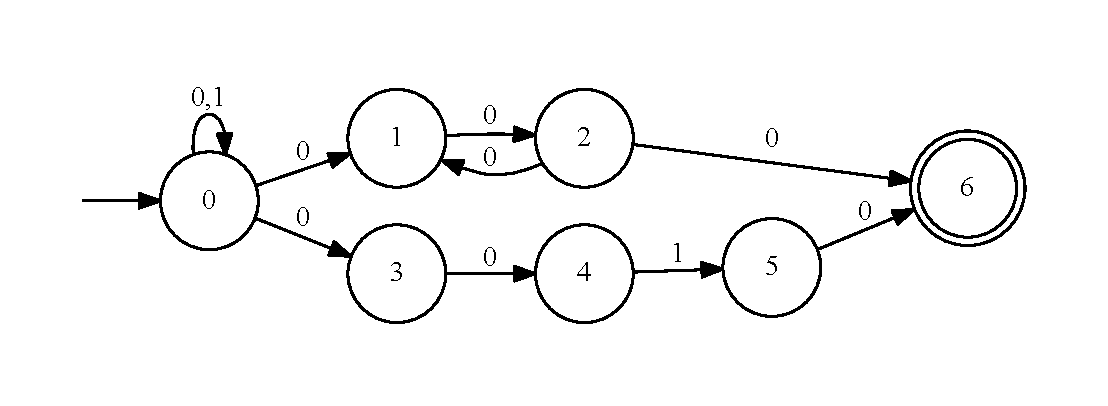
\includegraphics[width=\textwidth]{bilder/nfa_beispiel.pdf}
	\caption{Visuelle Darstellung des NFAs zum regulären Ausdruck \texttt{(0|1)*((00)+|001)0}}
	\label{nfa_beispiel}
\end{figure}

\begin{figure}[ht]
	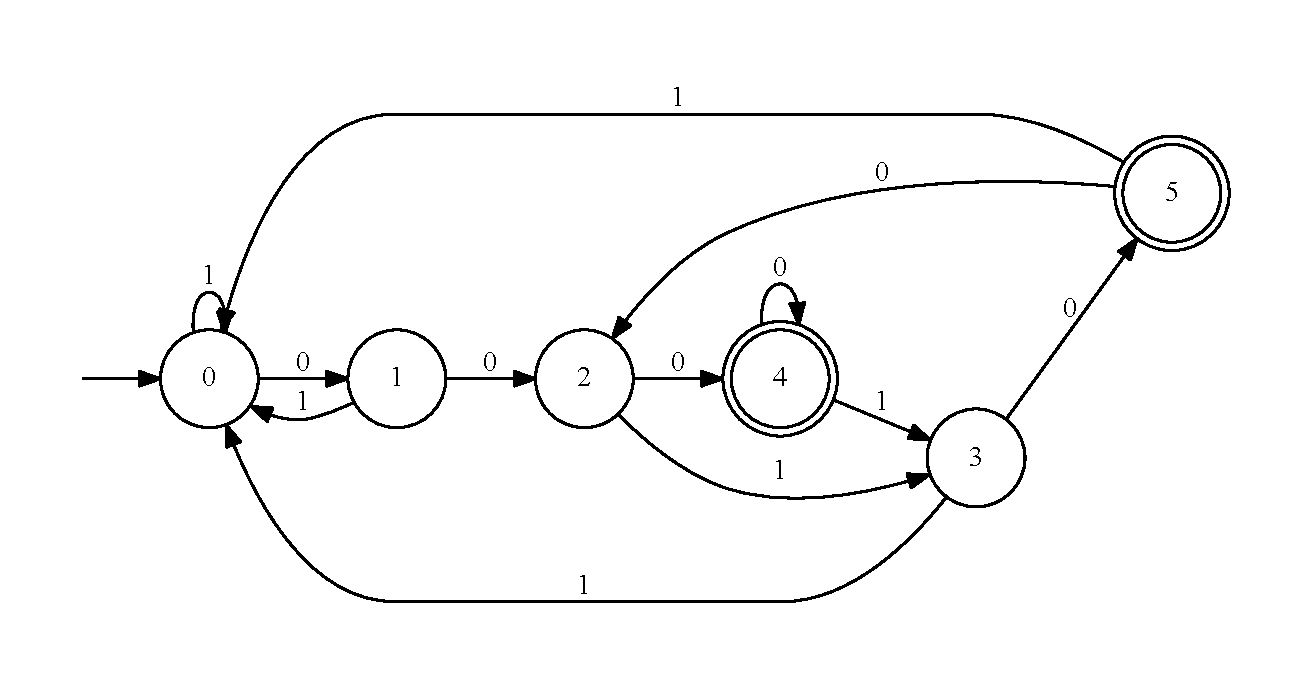
\includegraphics[width=\textwidth]{bilder/dfa_beispiel.pdf}
	\caption{Visuelle Darstellung des DFAs zum regulären Ausdruck \texttt{(0|1)*((00)+|001)0}}
	\label{dfa_beispiel}
\end{figure}

\section{Durchführung eines Musterabgleichs}

Der vorgestellte DFA lässt sich als zweidimensionale Übergangstabelle darstellen, die für einen gegebenen Ausgangszustand und ein gelesenes Eingabezeichen den Folgezustand zurückliefert.
Beginnend mit dem Startzustand muss somit lediglich für jedes Zeichen des Eingabewortes der aktuelle Zustand entsprechend der Tabelle angepasst werden und es kann am Ende überprüft werden, ob ein akzeptierender Zustand erreicht wurde.
Dieses Verfahren wird in Listing \ref{dfa_matching} schematisch dargestellt.

\begin{lstlisting}[language=Python,
caption=Durchführung des Musterabgleichs mithilfe eines DFA,
label=dfa_matching]
dfa = [[1, 0],
	[2, 0],
	[4, 3],
	[5, 0],
	[4, 3],
	[2, 0]]
cs = 0
accepting = [4, 5]

word = "010010"

for c in word:
	cs = dfa[cs][int(c)]

if cs in accepting:
	print("Word matches regular expression!")
\end{lstlisting}

\begin{lstlisting}[language=Python,
caption=Durchführung des Musterabgleichs mithilfe eines NFA,
label=nfa_matching]
nfa = [[[0, 1, 3], [0]],
	[[2], []],
	[[1, 6], []],
	[[4], []],
	[[], [5]],
	[[6], []],
	[[], []]]
cs = [0]
accepting = [6]

word = "010010"

for c in word:
	newCs = []
	for s in cs:
		newCs = newCs + nfa[s][int(c)]
	cs = newCs

for s in cs:
	if s in accepting:
		print("Word matches regular expression!")
		break
\end{lstlisting}

Listing \ref{nfa_matching} stellt entsprechend das Verfahren zur Durchführung des Musterabgleichs mittels eines NFAs dar.
Dieses funktioniert sehr ähnlich zu einem DFA, allerdings müssen gegebenenfalls mehrere Zustände gleichzeitig betrachtet werden, wodurch die Auswertung des Automaten komplizierter und zeitaufwändiger wird.

\section{Auswahl eines geeigneten Ansatzes}

Der Nachteil bei der Verwendung von NFAs liegt darin, dass teilweise mehrere Zustände gleichzeitig aktiv sind, da verschiedene Pfade auf einmal verfolgt werden müssen.
Dadurch steigt die Rechenlast beim Lesen von Zeichen und die allgemeine Performanz sinkt.
Bei DFAs ist dies nicht der Fall, da durch den Determinismus zu jeder Zeit klar ist, welche Transition verfolgt werden muss und in welchem Zustand der Automat sich befindet.

Der Nachteil eines DFA liegt allerdings darin, dass dieser im Gegensatz zum NFA eine exponentiell große Anzahl von Zuständen haben kann.
die Zeit für das Verarbeiten eines Strings wird dadurch zwar nicht direkt beeinflusst, allerdings steigt der Speicherverbrauch enorm, wodurch die Verwendung eines DFAs gegebenenfalls unmöglich wird.

Vergangene Arbeiten zeigen, dass ein unkomprimierter DFA die optimale Laufzeit erzielt \ref{Yu2013}.
Außerdem ist nicht zu erwarten, dass im Kontext einer Datenbankanfrage ein hoch komplexer regulärer Ausdruck benötigt wird, sodass der Automat eine effiziente Größe überschreiten würde.
Der exponentiellen Anzahl von Zuständen kann außerdem entgegen gewirkt werden, indem der Automat vor der Verwendung minimiert wird, was in den meisten Anwendungsfällen einen kompakten Automaten ergibt.

	\chapter{Ergebnis und Fazit}
	
	% Anhang
	\appendix
	\chapter{Umsetzung der String-Selektion mit Lane Refill}
\label{apx:equals_lane_refill}

\begin{lstlisting}[language=C++,
caption=Umsetzung der String-Selektion mit Lane Refill]
// shared memory for the divergence buffers
__shared__ int search_id_divergence_buffer[THREAD_COUNT];
__shared__ int current_divergence_buffer[THREAD_COUNT];

unsigned warpid = (threadIdx.x / 32);	// index of warp in block
unsigned bufferbase = (warpid * 32);    // buffer offset for warp in block
unsigned warplane = (threadIdx.x % 32); // index of lane in warp
unsigned prefixlanes = (0xffffffff >> (32 - warplane)); // previous lanes
int bufferelements = 0;        // number of elements in buffer

while(!flush_pipeline) {
	current = loop_var;
	
	/* execute previous operators in the pipeline */
	
	data_length = char_offset[current+1] - char_offset[current] - 1;
	
	// if string lengths are unequal, discard
	if (active && data_length != search_length)
		active = false;
	
	int numactive = __popc(__ballot_sync(ALL_LANES, active));
	while(bufferelements + numactive > THRESHOLD) {
	
		// refill empty lanes from buffer in case of underutilization
		if (numactive < THRESHOLD) {
			numRefill = min(32 - numactive, bufferelements);
			numRemaining = bufferelements - numRefill;
			
			previous_inactive = __popc(~__ballot_sync(ALL_LANES, active) & prefixlanes);
			
			if (!active && previous_inactive < bufferelements) {
				buf_ix = numRemaining + previous_inactive + bufferbase;
				search_id = search_id_divergence_buffer[buf_ix];
				current = current_divergence_buffer[buf_ix];
				active = true;
			}
			
			bufferelements -= numRefill;
		}
	
		int data_id = search_id + char_offset[current];
		
		// when strings don't match, inactivate the lane
		if (active && data_content[data_id] != search_string[search_id])
			active = false;
		
		search_id++;
		
		if (search_id == search_length) {
		
			/* execute following operators in the pipeline */
		
			active = false;
		}
		
		numactive = __popc(__ballot_sync(ALL_LANES, active));
	}
	
	// flush active lanes to buffer
	if (numactive > 0) {
		previous_active = __popc(__ballot_sync(ALL_LANES, active) & prefixlanes);
		buf_ix = bufferbase + bufferelements + previous_active;
		
		if(active) {
			search_id_divergence_buffer[buf_ix] = character_index;
			current_divergence_buffer[buf_ix] = current;
		}
		
		bufferelements += numactive;
		active = false;
	}
	
	loop_var += step;
}
\end{lstlisting}

	
	% Abbildungsverzeichnis
	\listoffigures
	\addcontentsline{toc}{chapter}{Abbildungsverzeichnis}
	\cleardoublepage
	
	% Literaturverzeichnis
	\printbibliography
	\addcontentsline{toc}{chapter}{\bibname}
	
	% Erklaerung
	\thispagestyle{myheadings}
	\markboth{}{ERKLÄRUNG}
	\addcontentsline{toc}{chapter}{Erklärung}
	% erklaerung.tex
\cleardoublepage
\normalsize
Hiermit versichere ich, dass ich die vorliegende Arbeit selbstständig verfasst habe und keine anderen als die angegebenen Quellen und Hilfsmittel verwendet sowie Zitate kenntlich gemacht habe.\\\\
Dortmund, den \today \\\\\\\\
Muster Mustermann
% EOF
	\cleardoublepage
\end{document}
